\section{Desenvolvimento Experimental}
\subsection{Materiais e Métodos}
Foi utilizado para o experimento o equipamento PASCO Modelo OS-8501 cosntituido por: 
\begin{itemize}
	\item Espelho fixo (M1);
	\item Espelho móvel (M2);
	\item Separador de feixes (\it{beam-splitter});
	\item Micrômetro;
	\item Câmara de vácuo.
\end{itemize}
Sendo utilizado também:
\begin{itemize}
	\item Lasers (um com comprimento de onda conhecido e outro a determinar);
	\item Lente divergente.
\end{itemize}

    O primeiro passo é alinhar o laser de comprimento de onda conhecido com o espelho móvel da base do interferômetro - é importante que o raio refletido seja desviado poucos milímetros do orifício do laser, evitando reflexões em seu interior. Após, insere-se a lente divergente entre o laser e o {\it beam-splitter}, posicionado a 45º de forma que o feixe seja parcialmente refletido para o espelho fixo, como consequência deve-se ver um padrão de franjas claras/escuras na superfície de projeção. Caso sejam formados dois padrões de franjas, deve-se ajustar o espelho fixo para que ambas se sobreponham. 

    Recomenda-se demarcar na superfície de projeção os limites de uma das franjas para facilitar a contagem durante o experimento, outra sugestão é a de se usar uma câmera fotográfica com filmagem em câmera lenta durante a contagem. 
    
Então é realizado a calibração do interferômetro utilizando o laser conhecido, inicialmente é posto a contagem do micrômetro no zero e então feito um deslocamento no espelho móvel utilizando a haste do micrômetro em 20 unidades, e contando quantas franjas são deslocadas é possível calibrar o interferômetro para que o comprimento de onda de qualquer laser possa ser encontrado.

O próximo estágio realizado é para se aferir o índice de refração do ar, é montado o equipamento com o laser de HeNe e antes do espelho fixo é posto uma câmara onde será feito vácuo, então o equipamento é alinhado novamento e variando a pressão na câmara de 10 em 10 mmMg é contado a variação das franjas. 	 
\subsection{Interpretação dos Resultados}
Após a realização da primeira parte do experimento, é encontrado que  cada variação do micrômetro equivale na verdade a $20,2 \times 10^{-6} m$. Substituindo o laser conhecido por um qualquer e utilizando a equação (\ref{eq:lbd}), é possivel encontrar o comprimento de onda do laser.

Para a segunda parte do experimento, foram repetidas as aferições para que o erro fosse reduzido, então com os dados de $\Delta P$ e $\Delta M$ e utilizando a equação (\ref{eq:ni}) são obtidos valores para a confecção do gráfico de $\eta \times \Delta P$ encontrado na figura (\ref{im:aa}).

 \begin{figure}[!h]
 	\centering
 		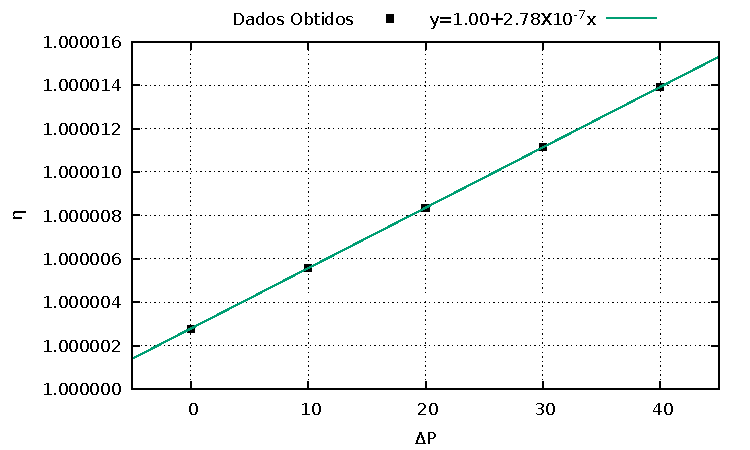
\includegraphics[scale= 1]{grafico/ar.pdf}
 	\caption{Interferômetro de Michelson}
 	\label{im:aa}
 \end{figure}

Assim 
\begin{equation*}
\alpha = \frac{\Delta m\lambda}{2d\Delta P}
\end{equation*}
\begin{equation*}
\alpha = 2.78\times 10^{-7}
\end{equation*}

Calculando o valor do coeficiente angular da reta é possivel encontrar o valor do índice de refração do ar, $\eta_{ar}$, aplicando o valor encontrado na equação (\ref{eq:ni}) e para este experimento foi encontrado $\eta_{exp} = 1.00002052$.

Comparando o valor obtido com o teórico que vale $\eta_{ar} = 1.000293$ é encontrado um desvio percentual de $D\% = 0,0272\%$.
